\bluepage{OpenGL}

\begin{frame}\frametitle{OpenGL}
\scriptsize
\begin{itemize}
\item OpenGL Open Graphics Language (Library) 
\item OpenGL is API for 3D graphics and general purpose computing (GPGPU).
\item It's origin is IrisGL by SGI
\item Multiplatform
\item Can be used from almost any language .
\item OpenGL shading language
\end{itemize}

\begin{itemize}
\item OpenGL Open Graphics Language (Library) 
\item OpenGL je API pro 3D grafiku a obecké výpočty na GPU.
\item Vychází z IrisGL od SGI 
\item Platformně nezávislé 
\item Použitelné skoro z každého jazyka 
\item Obsahuje vlastní jazyk GLSL pro programování GPU
\end{itemize}
  \begin{figure}[h]
  \includegraphics[width=5cm,keepaspectratio]{pics/opengl/logo}
  \end{figure}
\end{frame}

\begin{frame}\frametitle{Why to use OpenGL / OpenGL - proč používat?}
\scriptsize
\begin{itemize}
  \item{Linux, Window, Mac Os X, Android,...}
  \item{C, C++, Python, Java, Javascript, ...}
  \item{OpenGL is backward compatible}
  \item{OpenGL is low levels API (not as low as Vulkan)}
  \item{OpenGL has simple API}
  \item{OpenGL is fast (if used properly)}
  \item{OpenGL is open industrial standard}
  \item{WebGL}
\end{itemize}

\begin{itemize}
  \item{OpenGL je multiplatformní - Linux, Window, Mac Os X, Android,...}
  \item{OpenGL lze použít téměř z každého jazyka - C, C++, Python, Java, Javascript, ...}
  \item{OpenGL je zpětně kompatibilní}
  \item{OpenGL je nízkoúrovňové (Vulkan je nízko úrovňovější)}
  \item{OpenGL má jednoduché API}
  \item{OpenGL je rychlé (když se správně použije)}
  \item{OpenGL je otevřený industriální standard}
  \item{WebGL}
\end{itemize}
\end{frame}


\begin{frame}\frametitle{OpenGL versions / Verze OpenGL}
  \scriptsize{
\begin{itemize}
\item{OpenGL}
\begin{itemize}\scriptsize
\item 1.x - Fixed pipeline / fixní pipeline
\item \textbf{2.x} - Programable pipeline / programovatelná pipeline
\item 3.x - geometry shader, \textbf{Deprecation}
\item 4.x - Hardware tessellation, double precision / Hardwarová tesselace, dvojitá přesnost
\item 4.3 - Compute shaders / Compute shadery
\item 4.5 - Direct State Access
\item 4.6 - SPIRv
\end{itemize}

\item{OpenGL ES}
\begin{itemize}\scriptsize
\item Embeded systems, mobiles, tables / Vestavěné systémy, mobily, tablety
\item 1.x - Fixed pipeline / fixní pipeline
\item \textbf{2.x} - programable pipeline / programovatelná pipeline
\item 3.x - Occlusion queries, 3D textury, transform feedback
\end{itemize}

\item{WebGL}
\begin{itemize}\scriptsize
\item OpenGL in internet browser / OpenGL ve webovém prohlížeči
\item \textbf{Very similar to OpenGL ES / Velmi podobné OpenGL ES}
\end{itemize}

\end{itemize}
  }
\end{frame}

\begin{frame}\frametitle{OpenGL}
\scriptsize
\begin{itemize}
  \item OpenGL architecture is client-server
  \item Application runs on CPU and calls OpenGL function to access GPU
  \item Command Queue is hidden
\end{itemize}

\begin{itemize}
  \item OpenGL je architektura klient server
  \item Aplikace běží na CPU a využívá OpenGL pro přístup k GPU
  \item Front příkazů mezi CPU a GPU je skryta
\end{itemize}
\begin{figure}[h]
  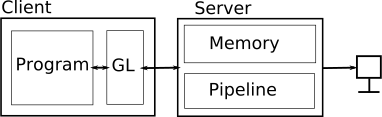
\includegraphics[width=10cm,keepaspectratio]{pics/opengl/clientserver}
\end{figure}
\end{frame}

\begin{frame}
\frametitle{OpenGL}
\begin{figure}[h]
	\includegraphics[width=14cm,keepaspectratio]{pics/opengl/RenderingPipeline}
\end{figure}
\end{frame}

\begin{frame}\frametitle{OpenGL API}
\scriptsize
\begin{itemize}
  \item Siple interface / Jednoduché rozhraní
    \begin{itemize}\scriptsize
      \item Only C functions / Pouze C funkce
      \item Data in form of numbers and arrays / Data jsou jen čísla a pole
      \item No structures, classes / Žádné struct, class
    \end{itemize}
  \item State machine / Stavový stroj
    \begin{itemize}\scriptsize
      \item Most of the commands set the state of pipeline / Většina příkazů nastavuje stav pipeline
      \item State cannot change on its own / Stav se sám nemění
    \end{itemize}
  \item OpenGL (Rendering) Context
    \begin{itemize}\scriptsize
      \item Main object of OpenGL / Hlavní objekt OpenGL
      \item Must be created outside of OpenGL / Mimo OpenGL (WGL/GLX)
      \item Encapsulates data, state, connection to the output / Zapouzdřuje data, stav, napojení na výstup
    \end{itemize}
\end{itemize}
\end{frame}

\begin{frame}[fragile]\frametitle{Commands and types / Příkazy a typy}
  glName{\it NT}(...)
  \begin{itemize}
    \item N - number of parameters / počet parametrů
    \item T - type of parameters / typ parametrů
  \end{itemize}
    \begin{tabular}{l|l|l|l}
    b & 8b integer & signed char & GLbyte \\ 
    s & 16b integer & short & GLshort \\ 
    i & 32b integer & long & GLint,GLsizei \\ 
    f & 32b float & float & GLfloat,GLclampf \\ 
    d & 64b float & double & GLdouble,GLclampd \\ 
    ub & 8b unsigned & unsigned char & GLubyte,GLboolean \\ 
    us & 16b unsigned & unsigned short & GLushort \\ 
    ui & 32b unsigned & unsigned long & GLuint,GLenum,GLbitfield \\ 
    *v & pointer * & & \\
    \end{tabular}
\begin{minted}[bgcolor=bg]{packages/c_cpp.py:CppLexer -x}
GLvoid glUniform2f(GLuint,GLfloat,GLfloat);
GLvoid glUniform2fv(GLuint,GLfloat*);
\end{minted}
\end{frame}

\begin{frame}\frametitle{Příkazy a typy}
\scriptsize
OpenGL commands can be divided into several groups.
\begin{itemize}
  \item \textbf{Commands for OpenGL object management (10 main OpenGL objects)}
  \item \textbf{Execution commands (draw commands, compute commands)}
  \item \textbf{State commands (set OpenGL state)}
  \item Debug commands
  \item Framebuffer commands
  \item Synchronization commands (glFinish)
  \item Util commands
\end{itemize}

OpenGL příkazy lze rozdělit do několika skupin
\begin{itemize}
  \item \textbf{Příkazy pro správu OpenGL objektů (10 hlavních OpenGL objektů)}
  \item \textbf{Exekuční příkazy (kreslící a výpočetní příkazy)}
  \item \textbf{Stavové příkazy (nastavují globální stav OpenGL, příkazy pro zjištění stavu)}
  \item Debugovací příkazy
  \item Operace s framebufferem
  \item Příkazy pro synchronizaci (glFinish)
  \item Utilitní příkazy
\end{itemize}
\end{frame}


\begin{frame}\frametitle{OpenGL Objekty}
  \scriptsize
  GLvoid glCreate{\it Objects}(GLsizei n,GLuint * objects);\\
  GLvoid glDelete{\it Objects}(GLsizei n,const GLuint * objects);

  \begin{itemize}
    \item Object name - GLuint, all OpenGL object instances are represented with integer
    \item 0 is reserved for empty object
  \end{itemize}

  \begin{itemize}
    \item Jméno objektu - GLuint, všechny objekty jsou v API reprezentovány integerem
    \item 0 rezervována pro prázdný objekt
  \end{itemize}

  Objects / Objekty:
  \begin{itemize}
    \item \textbf{Program}
    \item \textbf{Shader}
    \item \textbf{Buffer}
    \item \textbf{Vertex Array Object}
    \item Texture
    \item Framebuffer
    \item Renderbuffer
    \item Sampler
    \item Asynchronous Query
    \item ProgramPipeline
  \end{itemize}
\end{frame}

\begin{frame}\frametitle{Drawing with OpenGL / Kreslení pomocí OpenGL}
\scriptsize
  For drawing, it is necessary to initialize several OpenGL objects (Shaders, Shader Programs, Buffers, Vertex Arrays), set OpenGL state and execute draw command.
  \begin{enumerate}
    \item Compile and link shader programs from string
    \item Allocate buffers and copy data from CPU
    \item Setup vertex array object to tell OpenGL about the layout of the data in buffers
    \item Setup OpenGL state
    \item Execute draw call
  \end{enumerate}

  Pro kreslení je potřeba inicializovat několik OpenGL objektů (Shadery, Shader Programy, Buffery, Vertex Array objekty), nastavit OpenGL stav a zavolat kreslící příkazy.
  \begin{enumerate}
    \item Zkompilování a slikování shader programů z řetězce
    \item Alokace bufferu a nakopírování dat z CPU
    \item Nastavení vertex array tak, aby popisoval formát dat v bufferech
    \item Nastavení OpenGL stavu
    \item Spuštění kreslícího příkazu
  \end{enumerate}
\end{frame}


